%%% Autor: 	Max Beining
%%% VORLAGE 

%% ALLGEMEINE EINSTELLUNGEN -------------------------------
\documentclass[11pt, a4paper, DIV=12]{scrartcl}
\usepackage[T1]{fontenc}
\usepackage[utf8]{inputenc}
\usepackage[ngerman]{babel}
%----------------------------------------------------------
%% ZUSATZPAKETE					% Verwendung (Bsp.)
\usepackage{caption}			% ...
\usepackage{enumitem}			% Aufzaehlung Abstand 0pt
\usepackage{nicefrac}
\usepackage{graphicx}


%% TABELLEN- UND ABBILDUNGEN NAME -------------------------
\captionsetup[figure]{justification=centerlast}
\captionsetup[table]{justification=centerlast}
\KOMAoption{captions}{tableheading}
\renewcaptionname{ngerman}{\figurename}{Abb.}
\renewcaptionname{ngerman}{\tablename}{Tab.}
\addtokomafont{caption}{\small}
\setcapindent{0pt}
%----------------------------------------------------------

\usepackage{here}

%==============================================================================
%------------------------------BEGINN DES HAUPTEILS ---------------------------
%==============================================================================
\begin{document}%%%%%%%%%%%%%%%%%%%%%%%%%%%%%%%%%%%%%%%%%%%%%%%%%%%%%%%%%%%%%%%

\noindent
\textbf{Universität Leipzig, WS~20/21} \vspace*{-0.25cm}
\section*{\underline{Modellierung und Programmierung 1}}
\subsection*{Übungsserie 1: Modellierung mit UML}
\noindent
Lösung erstellt von: Max Beining \\
\rule{\linewidth}{1pt} \\

%--------------------------------------

\subsubsection*{Aufgabe 1: UML-Klassendiagramm \glqq Werkstatt\grqq}
\begin{figure}[h]
	\centering
	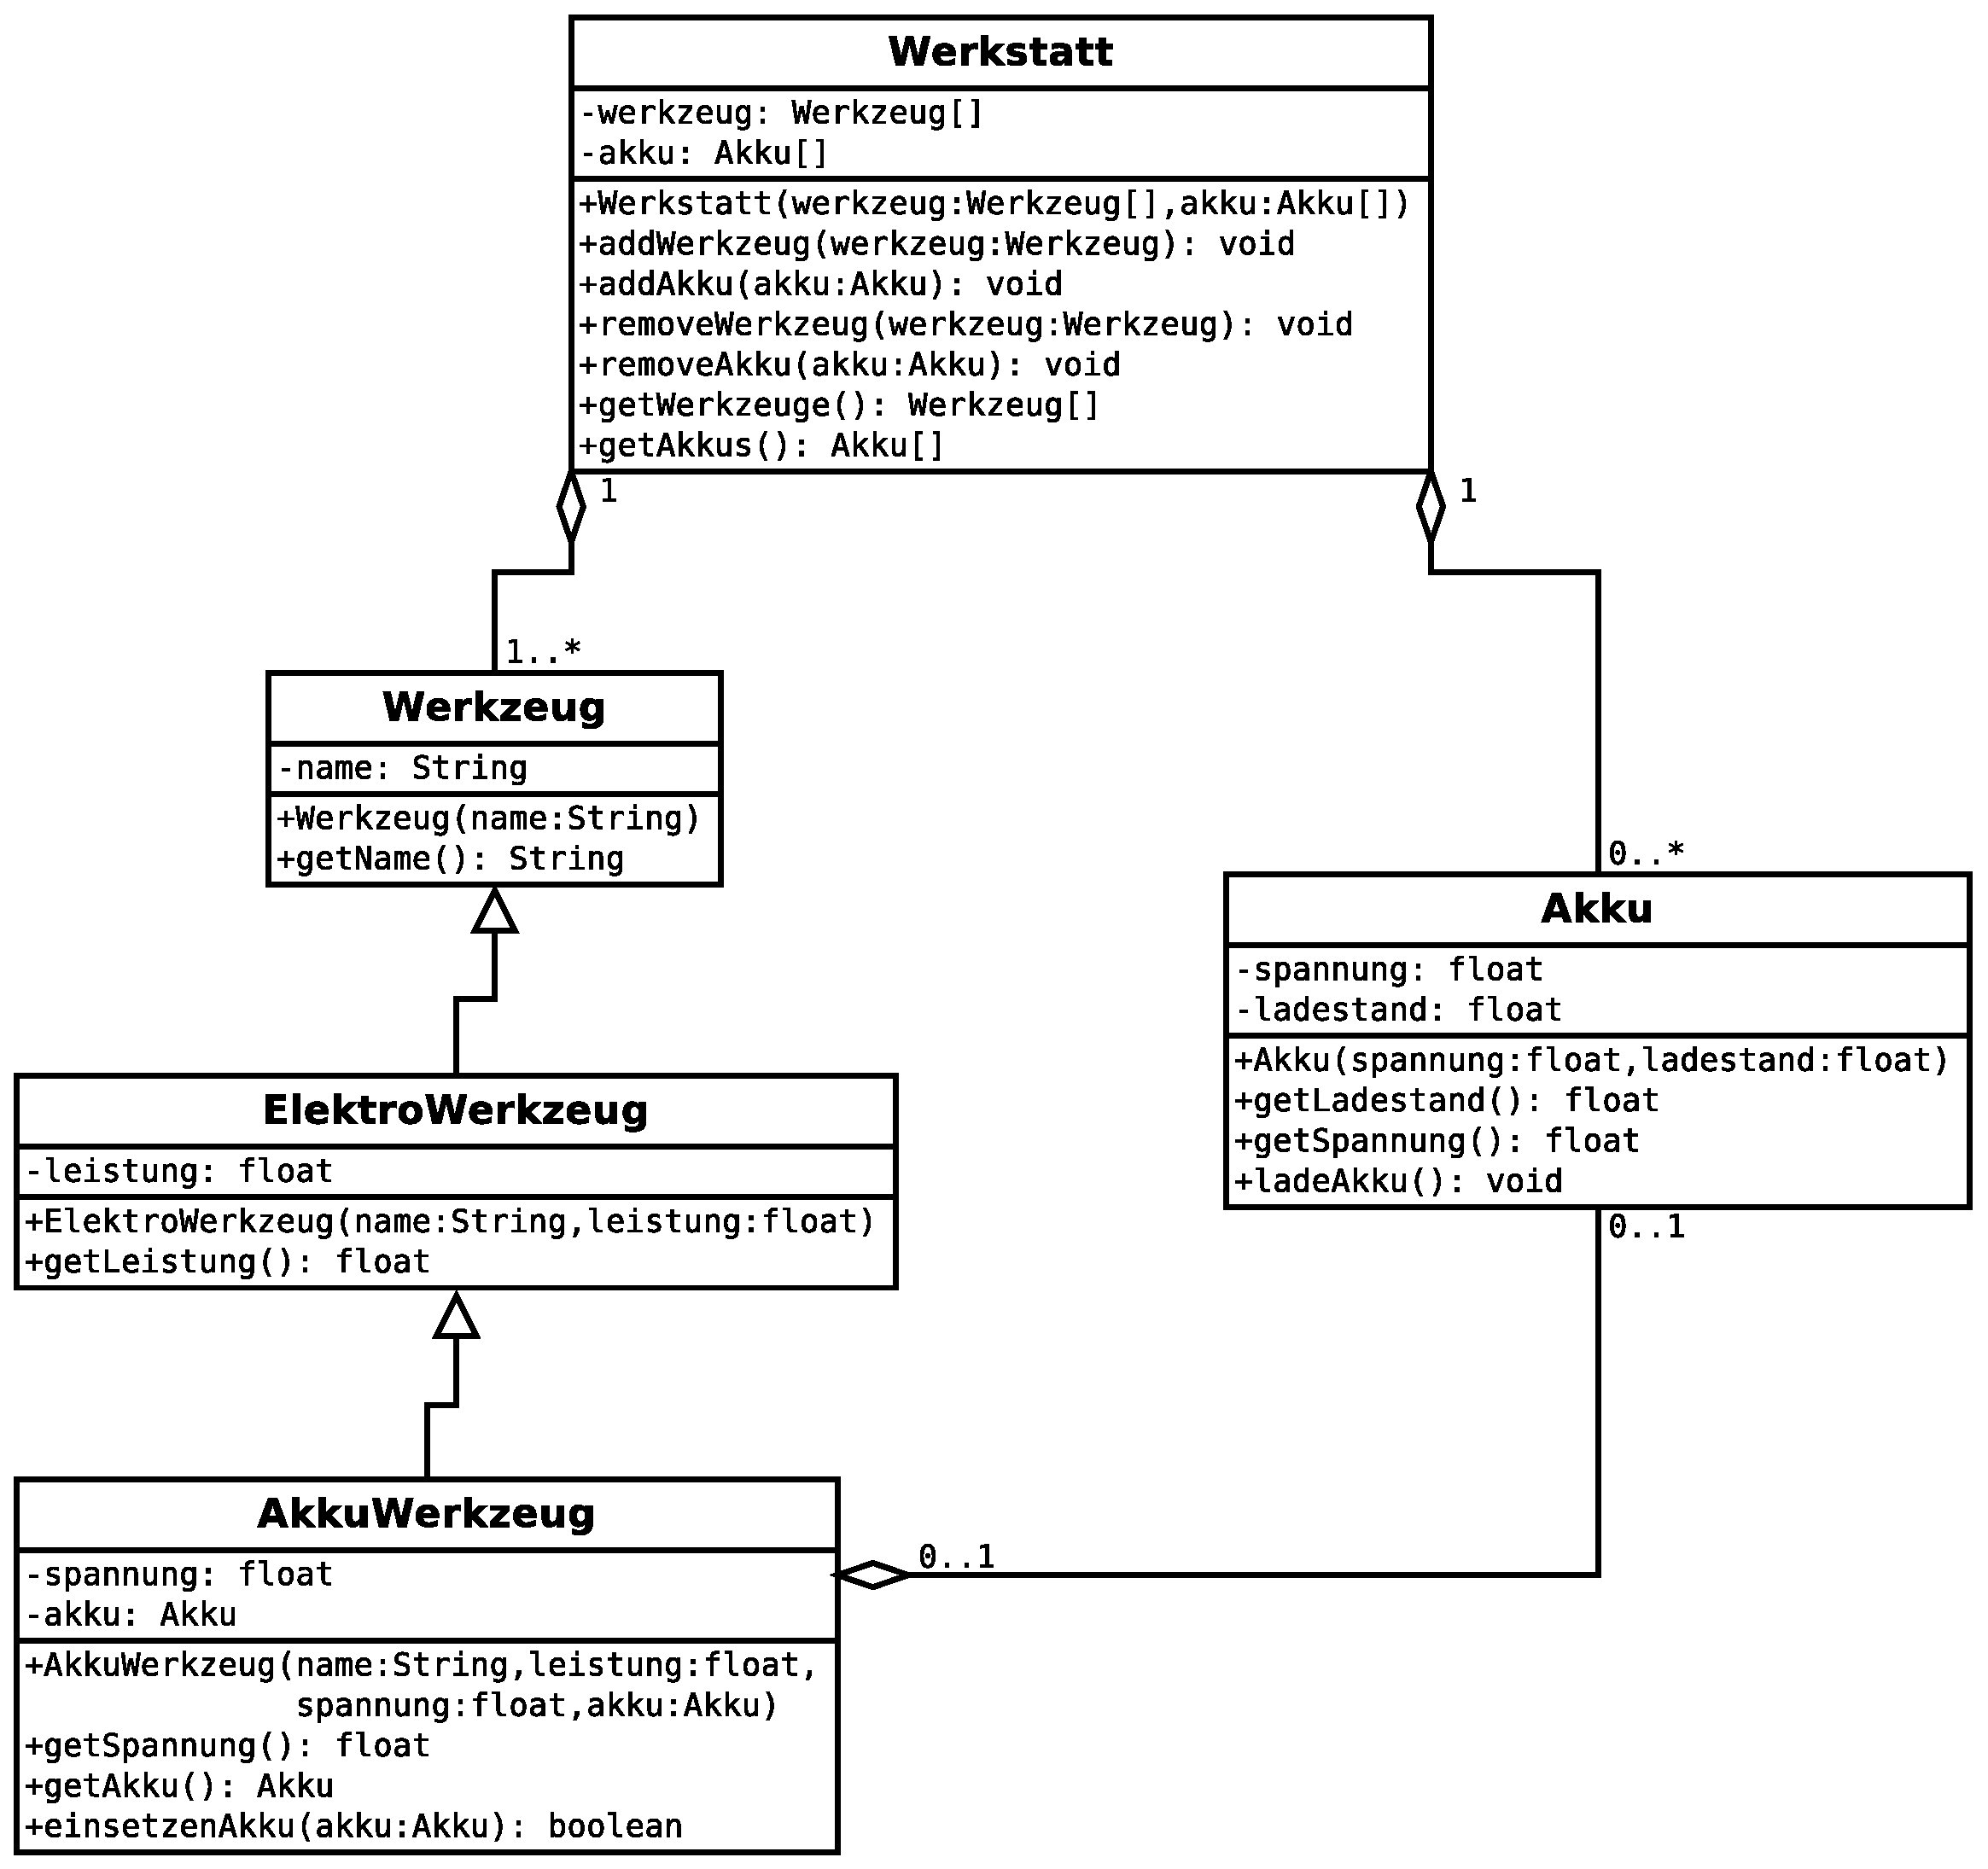
\includegraphics[width=\linewidth]{uebung01_werkstatt.eps}
\end{figure}

\clearpage
\subsubsection*{Aufgabe 2: UML-Klassendiagramm \glqq Hotel\grqq}
\begin{figure}[h]
	\centering
	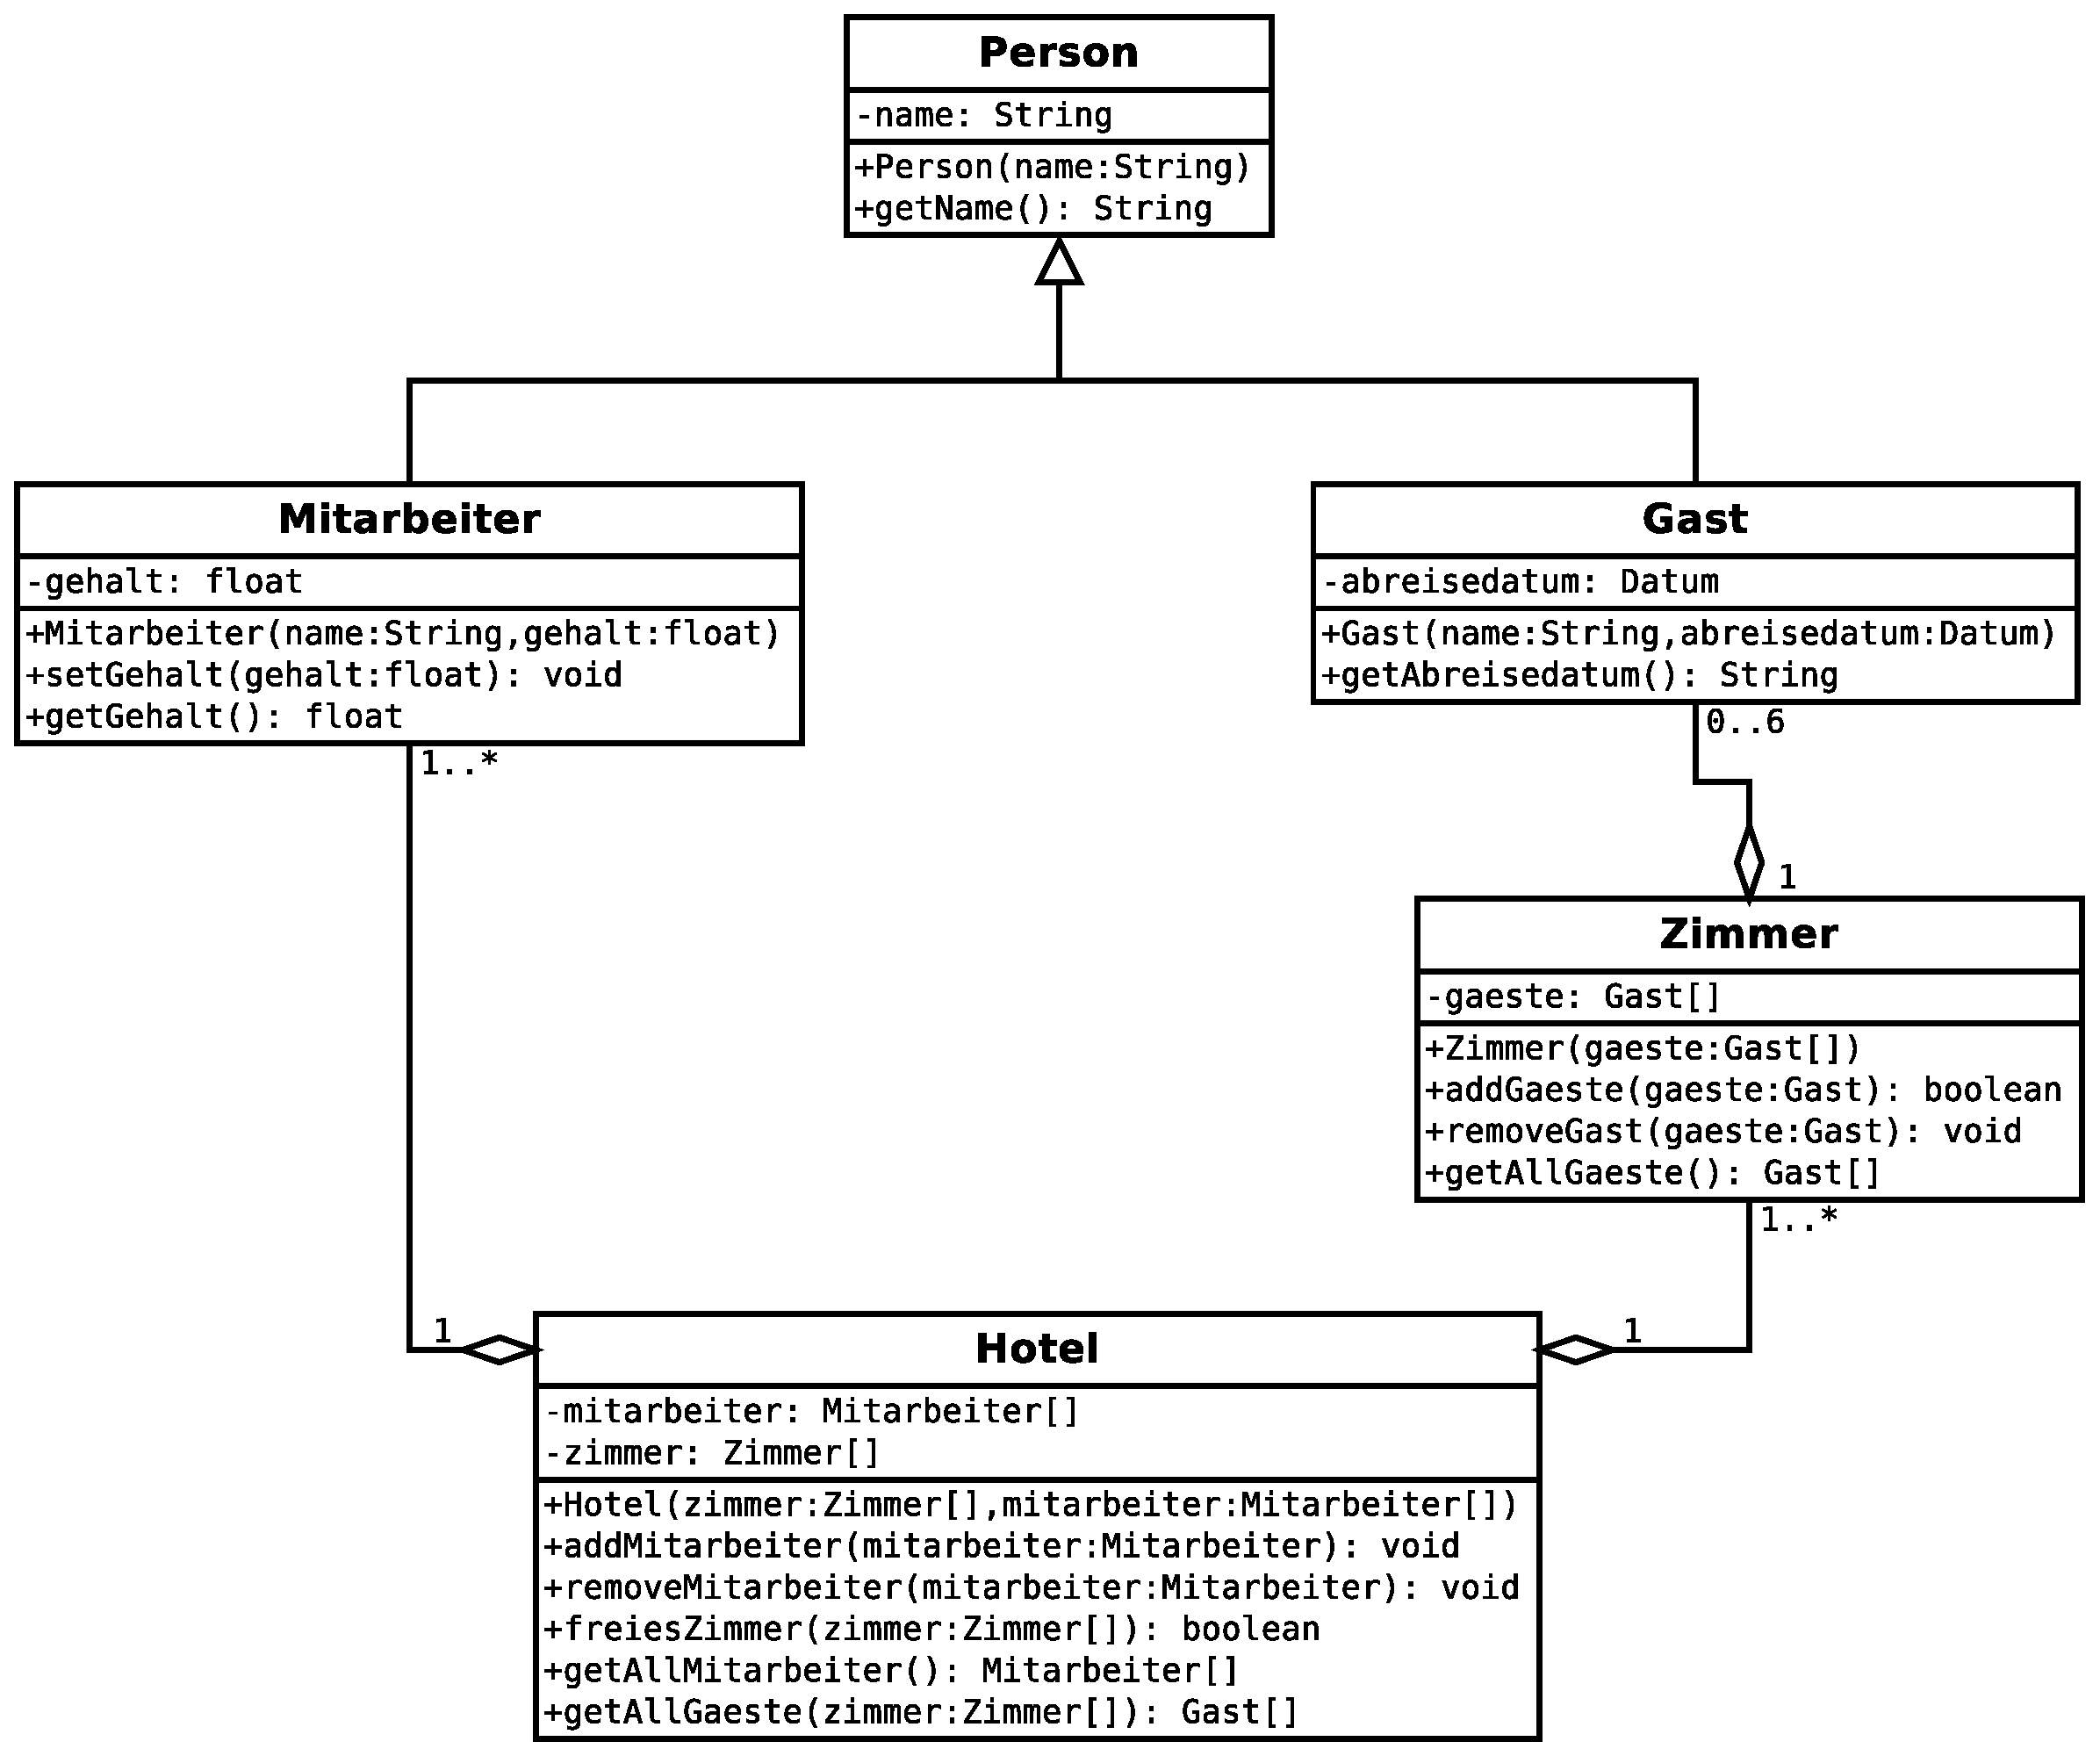
\includegraphics[width=\linewidth]{uebung01_hotel.eps}
\end{figure}
%


%==============================================================================
%------------------------------ENDE DES HAUPTEILS -----------------------------
%==============================================================================
\end{document}%%%%%%%%%%%%%%%%%%%%%%%%%%%%%%%%%%%%%%%%%%%%%%%%%%%%%%%%%%%%%%%%%
